\documentclass[
DIV10,              % Seite in X K�stchen einteilen (Seihe Koma-Script Guide)
%DIVcalc,           % Besten DIV Wert berechnen (Seihe Koma-Script Guide)
fontsize=12pt,      % Schriftgr��e 12 Punkte
oneside,            % Einseitig
parskip,            % Paragraphen nicht einr�cken
headsepline,        % Kopfzeile nach unten durch Linie abgrenzen (scrheadings)
%footbotline,       % Fusszeile nach unten durch Linie abgrenzen (scrheadings)
plainheadsepline,   % Kopfzeile nach unten durch Linie abgrenzen (scrplain)
plainfootbotline,   % Fusszeile nach unten durch Linie abgrenzen (scrplain)
%headtopline,       % Kopfzeile nach oben durch Linie abgrenzen (scrheadings)
footsepline,        % Fusszeile nach oben durch Linie abgrenzen (scrheadings)
plainheadtopline,   % Kopfzeile nach oben durch Linie abgrenzen (scrplain)
plainfootsepline,   % Fusszeile nach oben durch Linie abgrenzen (scrplain)
headexclude,        % Kopfzeile nicht als Teil des Inhalts setzen
footexclude,        % Fusszeile nicht als Teil des Inhalts setzen
bibtotocnumbered,   % Literaturverzeichnis nummeriert ins Inhaltsverzeichnis aufnehmen
%bibtotoc,          % Literaturverzeichnis ins Inhaltsverzeichnis aufnehmen
liststotocnumbered, % Sonstige Verzeichnise nummeriert ins Inhaltsverzeichnis aufnehmen
%liststotoc,        % Sonstige Verzeichnise ins Inhaltsverzeichnis aufnehmen
idxtotocnumbered    % Index nummeriert ins Inhaltsverzeichnis aufnehmen
%idxtotoc           % Index ins Inhaltsverzeichnis aufnehmen
]{scrbook}          % Koma-Script Klasse zum setzen eines Buchs

% Package um Zeilenabstand zu steuern
\usepackage{setspace}
\usepackage{upgreek}
 
%Einstellungen der Seitenr�nder
% for twoside
%\usepackage[inner=2cm,outer=4cm,top=2cm,bottom=2cm,includeheadfoot]{geometry}
% for oneside
%\usepackage[left=4cm,right=2cm,top=2cm,bottom=2cm,includeheadfoot]{geometry}
%\usepackage{geometry}
%\geometry{bindingoffset=40mm,top=20mm,textheight=245mm,textwidth=160mm,heightrounded,right=20mm,head=14.5pt}

% F�r nicht globale Seitenr�nder
\usepackage{anysize}
\usepackage{geometry}
\geometry{textwidth=150mm}

% Die "Standard-Header" f�r deutsche Dokumente
\usepackage[latin1]{inputenc}    % ISO-8859-1 bzw. Latin1 als Encoding
\usepackage[T1]{fontenc}         % T1 Schriften verwenden (sieht besser aus)
%\usepackage[ngerman]{babel}      % Neue deutsche Rechtschreibung und �bersetzungen

% "Sch�nere" Schriften einbinden
\usepackage{mathpazo}            % Serifen-Font mit passendem Math-Font
\usepackage[scaled=.95]{helvet}  % Serifenloser Font passend zu mathpazo
\usepackage{courier}             % "Sch�nerer" Festbreiten-Font

% Koma-Script Paket zum setzen vom Kopf- und Fusszeilen einbinden
\usepackage{scrpage2}
% Seitenstil f�r normale Seiten auf scrheadings setzen
% F�r Kapitelanfang und �hnliches wird scrplain verwendet
\pagestyle{scrheadings}
% Kopf- und Fusszeile l�schen
\clearscrheadfoot
% Automarkierungen verwenden \automark[rechts]{links}
% Statt \leftmark und \rightmark kann dann bei
% Koma-Script einfach \headmark verwendet werden
\automark[section]{chapter}
% Kopfzeile f�r scrplain und scrheadings setzen
% \*head[scrplain]{scrheadings}
%\ihead[Innen]{Innen}
%\chead[Mitte]{Mitte}
\ohead[\scshape\large\textbf{\headmark}]
{\scshape\large\textbf{\headmark}}
% Fusszeile f�r scrplain und scrheadings setzen
% \*foot[scrplain]{scrheadings}
\ifoot{Dionysios Satikidis}
%\cfoot[Mitte]{Mitte}
\ofoot[\pagemark]{\pagemark}
% Trennlinien f�r Kopf- und Fusszeile formatieren
% Siehe Optionen der Dokumentklasse
%\setheadtopline{2pt}
\setheadsepline{.4pt}
\setfootsepline{.4pt}
%\setfootbotline{2pt}

% Paket zum Einbinden von Quellcode als Listings
% Hinweis: UTF-8 Encoding f�hrt zu Problemen mit Umlauten
\usepackage{listings}

\usepackage{color}

% F�r sidewaysfigure
\usepackage{rotating}

% Querformat
\usepackage{lscape}

% Mehrere Literaturverzeichnisse
\usepackage{multibib}
%Dio: 1.11.2010 habe die References entferent
%\newcites{bib,ref}{Bibliography,References}
\newcites{bib}{Bibliography}

% Caption package f�r Konfiguration von Textgr��e
\usepackage[small,bf]{caption}

%WORKAROUND F�R FEHLERHAFTES LISTINGS PAKET
\makeatletter
\@ifundefined{float@listhead}{}{%
    \renewcommand*{\lstlistoflistings}{%
        \begingroup
            \if@twocolumn
                \@restonecoltrue\onecolumn
            \else
                \@restonecolfalse
            \fi
            \float@listhead{\lstlistlistingname}%
            \setlength{\parskip}{\z@}%
            \setlength{\parindent}{\z@}%
            \setlength{\parfillskip}{\z@ \@plus 1fil}%
            \@starttoc{lol}%
            \if@restonecol\twocolumn\fi
        \endgroup
    }%
}
\makeatother

% Formatierung der Listings
\lstset{
captionpos=b,                % Beschriftung unterhalb (bottom)
numbers=left,                % Zeilennummern links
frame=trbl,                  % Rahmen zeichnen (top, right, bottom, left)
basicstyle=\small\ttfamily,  % Festbreitenschrift verwenden (small)
language=Java,               % Sprache auf Java einstellen
emph={function, require_once, \$this, print, parent, @author @package, @copyright, @name, @see, @access, @return, @var},
emphstyle=\color{black}\textbf,
numbers=left,
numberstyle=\tiny,
showstringspaces=false
}

% WORKAROUND F�R FOOTNOTES IN TABLES ----------------
\newcounter{myfootertablecounter}
%\setcounter{myfootertablecounter}{18}

\newcommand\myfootnotemark{%
%\refstepcounter{footnote}%
\addtocounter{footnote}{1}%
\footnotemark[\thefootnote]%
}%

\newcommand\myfootnotetext[1]{%
\addtocounter{myfootertablecounter}{1}
\footnotetext[\value{myfootertablecounter}]{#1}
}

% Abstand zwischen Kopfzeile und Kapitel�berschrift verringern
\renewcommand*{\chapterheadstartvskip}{\vspace{-1.8\baselineskip}} 

% ----------------------------------------------------

% Paket f�r PDF Metainformation
\usepackage[	pdftitle={Interim Report Master Thesis - Dionysios Satikidis, Brunel University West London},
		pdfauthor={Dionysios Satikidis},
		pdfsubject={Dissertation Interim Report Master Thesis},
		pdfkeywords={},
		plainpages=false,
		pdfpagelabels]{hyperref}

\usepackage{footnote}
\makesavenoteenv{tabular}

% Paket zur Erstellung von Stichwort- und Abk�rzungverzeichnissen einbinden
\usepackage[acronym=true, toc=true]{glossary}

% Format neu setzen
\setacronymnamefmt{\gloshort}
\setacronymdescfmt{\glolong}

% Symbolverzeichnis definieren (Erweiterung des Standardumfangs)
%\newglossarytype[slg]{symbolslist}{syg}{syi}
% Stichwortverzeichnis erstellen
%\makeglossary
% Abk�rzugsverzeichnis erstellen
\makeacronym
% Selbst definiertes Symbolverzeichnis erstellen
%\makesymbolslist
% Stil der einzelnen Verzeichnisse festlegen (Siehe glossary Dokumentation)
%\setglossarystyle[symbolslist]{style=long, number=none}
\setglossarystyle[acronym]{style=long, number=none}
%\setglossarystyle[glossary]{style=altlist, number=none}

% (Vor-) Definition von Eintr�gen f�r Stichwort-, Abk�rzungs- und Symbolverzeichnis
% Diese Befehle k�nnen auch mitten im Dokument benutzt werden
%\glossary{name={xyz}, description={...}}

\newacronym{UAV}{Unmanned Aerial Vehicle(s)}{}
\newacronym{HUAV}{Hovering Unmanned Aerial Vehicle(s)}{}
\newacronym{GUAV}{Gliding Unmanned Aerial Vehicle(s)}{}
\newacronym{MAV}{Micro Aerial Vehicle(s)}{}
\newacronym{DOF}{Degrees of Freedom}{}
\newacronym{IMU}{Inertial Measurement Unit}{}
\newacronym{MEMS}{Micro-Electro-Mechanical System}{}
\newacronym{HSE}{University of Applied Sciences Essslingen}{}
\newacronym{CCU}{Central Control Unit}{}
\newacronym{RF}{Radio Frequency}{}
\newacronym{SBC}{Single Board Computer(s)}{}
\newacronym{API}{Application Programming Interface(s)}{}
\newacronym{FPGA}{Field-Programmable Gate Array}{}
\newacronym{SLAM}{Simultaneous Localization And Mapping}{}
\newacronym{PID}{Proportional-Integral-Derivative}{}
\newacronym{MIMO}{Multiple-Input and Multiple-Output}{}
\newacronym{MBD}{Model Based Design}{}
\newacronym{HIL}{Hardware In the Loop}{}
\newacronym{MCU}{Microcontroller Unit}{}
\newacronym{DSP}{Digital Signal Processor}{}

%\symbolslist{name={$x$}, description={Eine ganzzahlige Variable, die das Ergebnis einer Berechnung darstellt}, sort=symbolpi}
%\symbolslist{name={$y$}, description={Eine ganzzahlige Variable, die als Parameter f�r eine Berechnung dient}, sort=symbolpi}

% Paket f�r Wortindex einbinden
\usepackage{makeidx}
% Wortindex erzeugen
\makeindex

% Paket zum generieren von Blindtext
%\usepackage{blindtext}

% Paket zum Einbinden von Bildern
\usepackage{graphicx}

% Beginn des eigentlichen Dokuments
\begin{document}

% Titelseite (verwendet pagestyle=empty)
\begin{titlepage}
% Seitenr�nder f�r die Titleseite
%\marginsize{left}{right}{top}{bottom} 
\marginsize{3cm}{3cm}{2cm}{2cm}
\begin{center}

\begin{tabular}{c}

\includegraphics[width=6cm]{graphic/Brunel_logo.png}\\
\end{tabular}

\vspace{0.5cm} \large School of Engineering \& Design -- Electronic \& Computer Engineering\\
\vspace{1cm} \Large MSc Distributed Computing Systems Engineering\\
\vspace{0.5cm} \Large Brunel University West London\\

\vspace{1.5cm} \Huge  Simulation and Performance Analysis\\ of a Distributed Position Correction\\
					  Scheme for Unmanned Aerial Vehicles \\
\vspace{0.5cm} \Large Interim Report\\
\vfill{}

\normalsize
\begin{tabular}{ll}
Author:      & Dionysios Satikidis\\[0.5cm]
Supervisor:  & Dr Marios Hadjinicolaou\\[0.5cm]
Date:        & 10/2010
\end{tabular}
\end{center}
\end{titlepage}

% Seitenr�nder f�r das Dokument
%\marginsize{left}{right}{top}{bottom} 
\marginsize{4cm}{2cm}{2cm}{2cm}

% "Frontmatter" beginnen (Formatierung umschalten)
% Platz f�r Inhaltsverzeichnis und anderes
\frontmatter

% Inhaltsverzeichnis ausgeben
\tableofcontents

% Stichwort- und Abk�rzungsverzeichnis ausgeben
%\def\glossaryname{Stichwortverzeichnis}
%\printglossary
\def\acronymname{List of Abbreviations}
\printacronym
%\def\symbolslistname{Symbolverzeichnis}
%\printsymbolslist

% Abbildungsverzeichnis ausgeben
\listoffigures
% Tabellenverzeichnis ausgeben
%\listoftables
% Das Listings-Verzeichnis scheint mit manchen Versionen vom Koma-Script
% bzw. des Listings Pakets nicht ohne weiteres zu funktionieren
%\lstlistoflistings

% ############################################################################################


% Hauptteil beginnen (Formatierung umschalten)
\mainmatter
\doublespacing
% -----------------------------------------------------------------------------------------

% PAGES: 5
\chapter{Introduction}
\label{mt:c:introduction}

%\begin{wrapfigure}{r}{5cm}
  %\centering
  %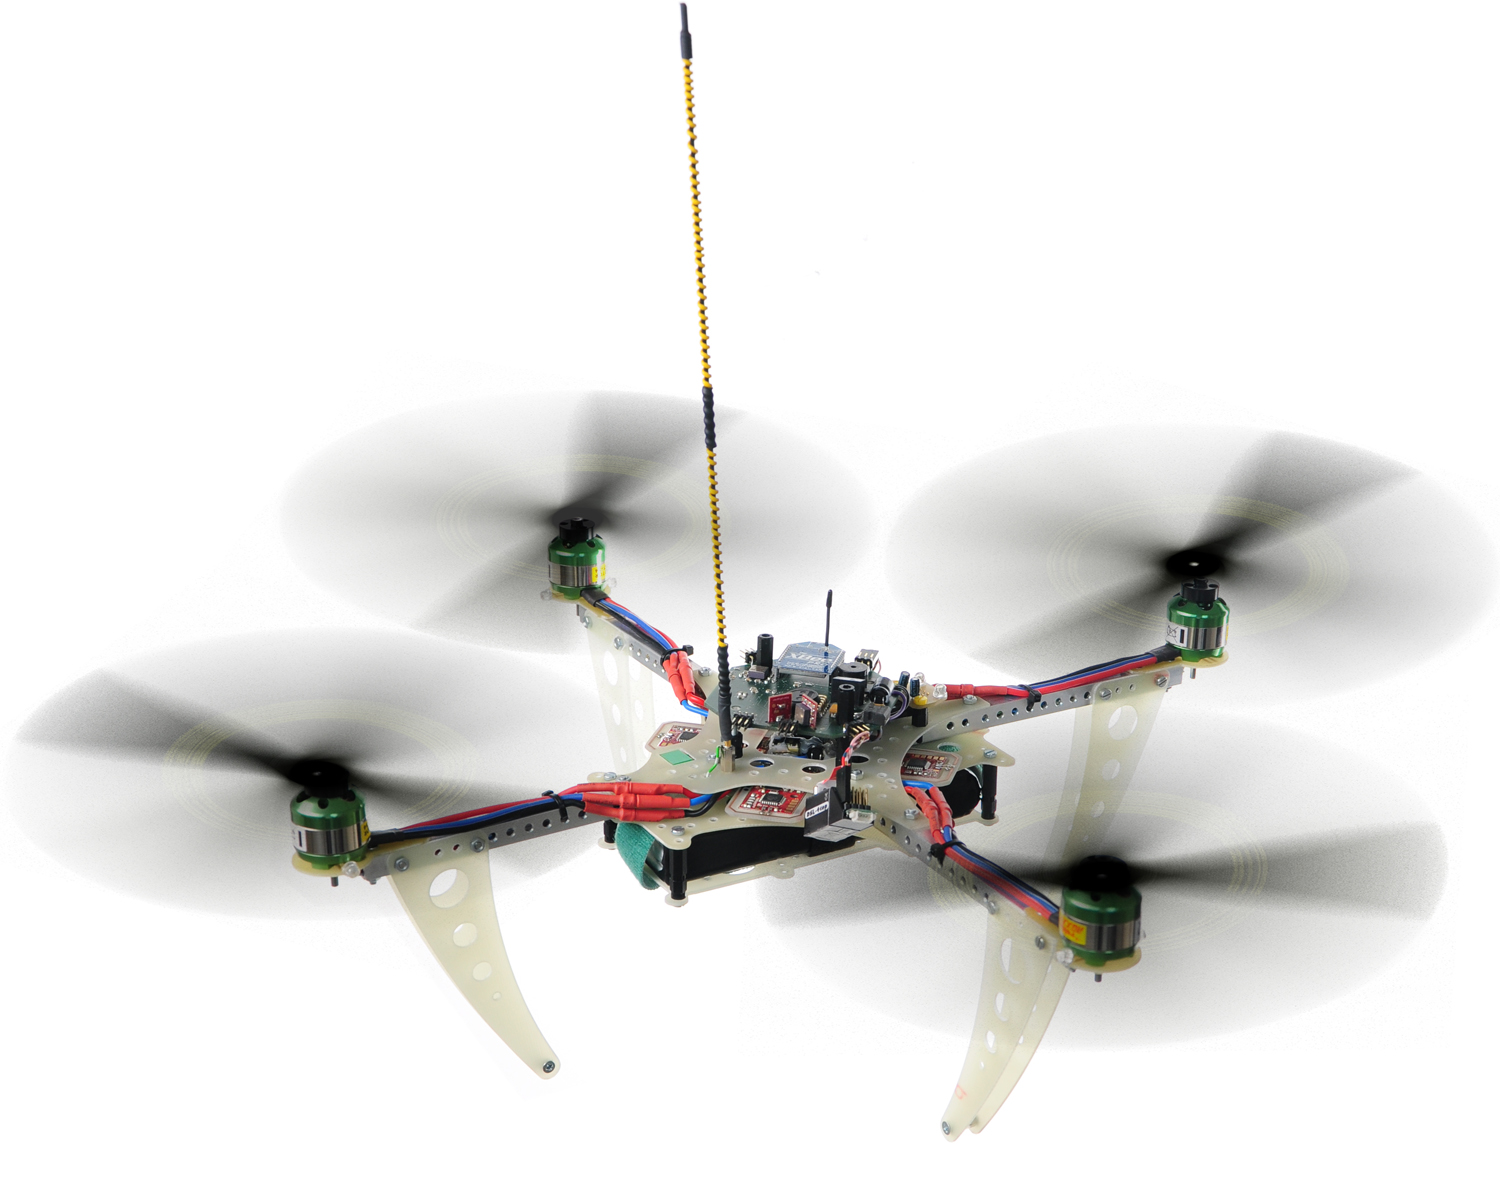
\includegraphics[width=0.5\textwidth]{graphic/QuadrocopterV3.jpg}
  %\caption {HSE Quadrocopter}
  %\label{fig:QuadrocopterV3.jpg}
%\end{wrapfigure}

In recent years, the interest in robotic science and the development of
robots enormously increased. Reasons for that are the unstoppable technological
progress in hard-and software techniques, but also the ambition to replace
humans with machines in dangerous, monotonous or unreachable industrial
environments (medical, space, aviation and so forth).
One area of these interests
is the aerial platform and the realization of \gls{UAV}, which are mostly controlled
via remote control or fly autonomous. These aircraft vehicles have several
capabilities, like in military or rescue operations, with special environments like
a burning house. For such indoor operation, it is important to
realise that some kinds of feedback sensors, like GPS-sensors, could not work
satisfactory. In such cases, \gls{UAV} face problems with their self-stabilization,
because their physical behaviour is generally unstable 
\citebib[p.1 Introduction]{BloWeiScaSie10}. Most of the attempts to stabilize
\gls{UAV} work with a clever combination of sensor equipment and control algorithms.
Mostly this controller uses an \gls{IMU} which is mounted on board and includes
acceleration sensors to detect movements in the given \gls{DOF}.
\newpage
Current acceleration
sensors, which are used for this purpose, are \gls{MEMS} or fiberoptic sensors which
have a finite precision and unacceptable error propagation in case of integration
for velocity or position detection 
\citebib[pp.11-13 Function Principles of MEMS, Sources of Error]{Fac08}.
 This problem also is a field of research for the Quadrocopter project of the
 \gls{HSE} \citebib[Website]{HSE10}. The goal of this Master's Thesis is to
research the topic of flight stabilisation and error drift elimination with an
optical sensor. This approach has to be tested and evaluated with the implementation of
a simulation focused on the behaviour of the flight dynamics in relation to the 
quality of the optical measurements and the control system of the quadrocopter.  

\begin{figure}[!h]
	\centering
		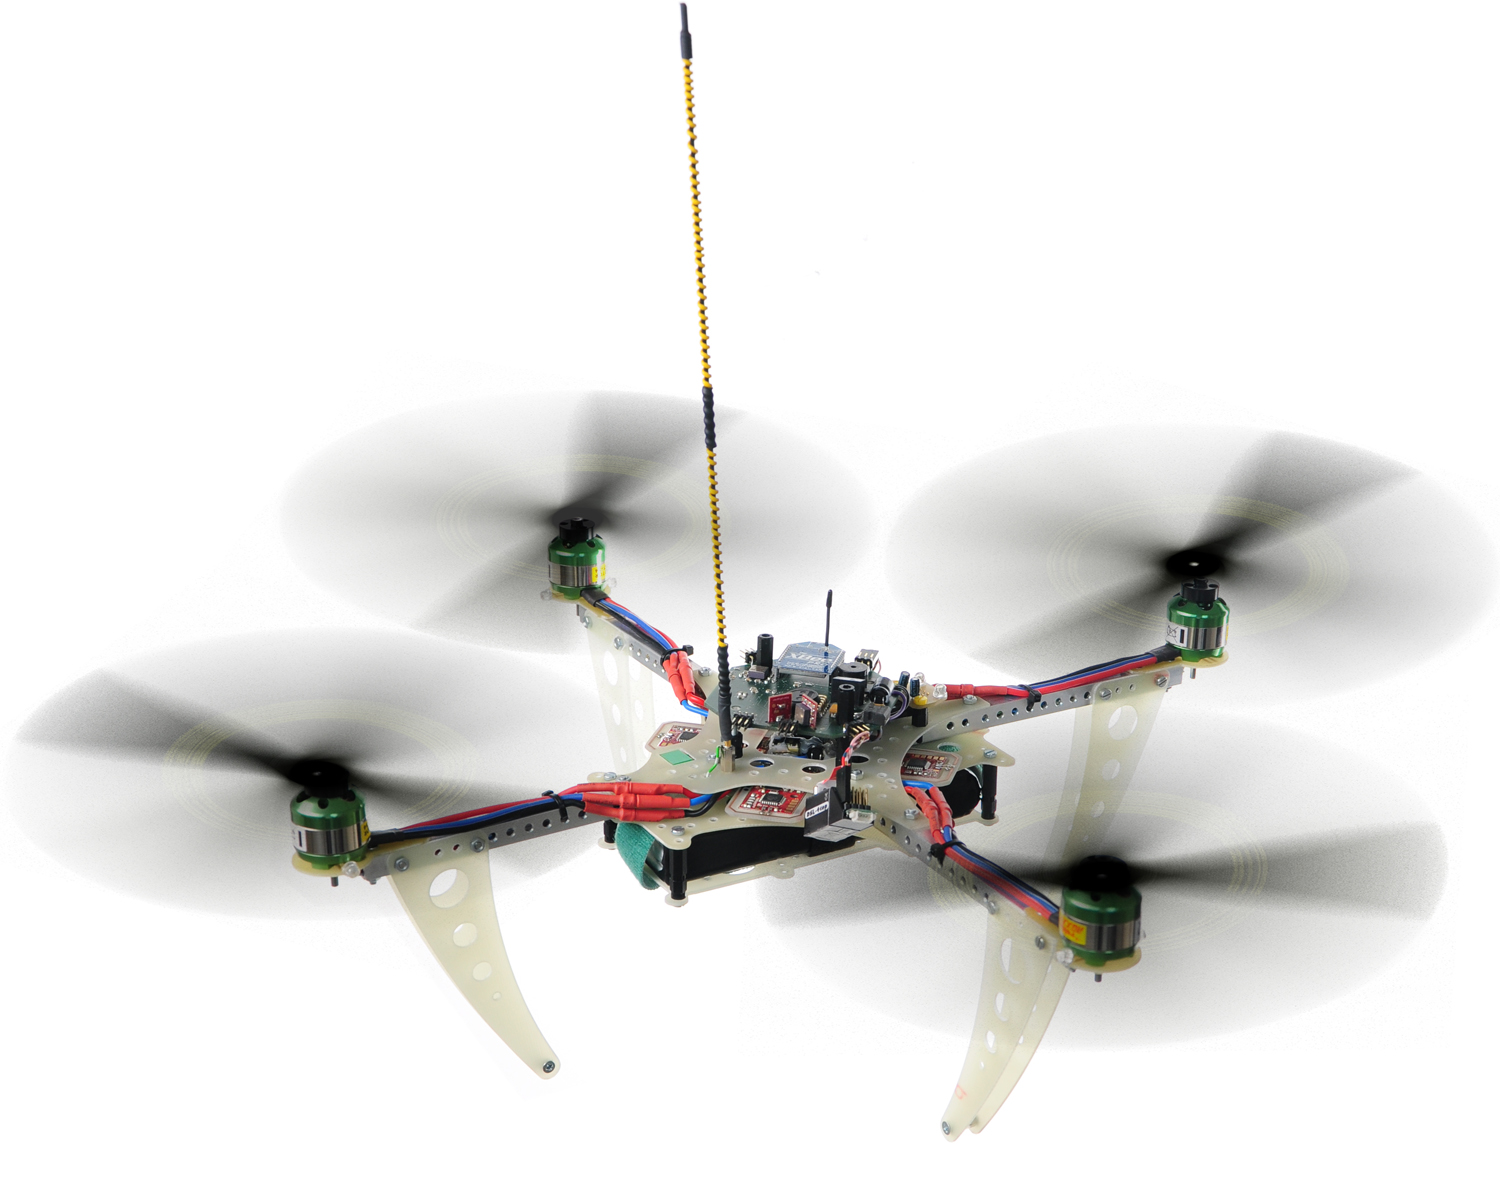
\includegraphics[width=0.8\textwidth]{graphic/QuadrocopterV3.jpg}
	\caption{HSE Quadrocopter}
	\label{fig:QuadrocopterV3.jpg}
\end{figure}

\newpage
\section{Context of the Project}

The quadrocopter project of the \gls{HSE} was launched with the goal to build a
system from the scratch, which is developed by students, scientific workers and
Professors. In a prior project, the \gls{PCB}, which contains
the parts necessary to control the quadrocopter, was designed by students at the
faculty of Mechatronics and Electrical Engineering in Goeppingen. Back then, these project
groups' focuses were on the simulation, implementation of basic functions
and visualization of the actual condition of the aircraft. The first two project
groups already show the their results, a multidisciplinary development
including hardware design, application development, embedded programming,
simulation and the interfaces between these special fields. In the year
2009, the Faculty of Information Technology adopted the development of the
project, with the aim to solve problems which came up in the previous development process
and to redesign the soft- and hardware architecture. So a new hardware design was
developed in a corporation between the two faculties, with the outcome of a \gls{CCU}
which can detect inertial movements in six \gls{DOF} and can control the four
actuators of the quadrocopter via so-called "brushless controllers".
One of the biggest unresolved problems so far is the development of a robust
controller and the elimination of drifts, which especially come up at the hovering state.
 The practice and experience of previous developments show that it is
indispensable to proof new developments with a simulation before they will be
realized at the real \gls{UAV}. So the main topic and focus of this Master's
Thesis will be on the development of a simulation that shows potential solutions
of the mentioned problems, and the research and evaluation for the outcome results.

\section{Problem Description}

Improvements in high density power storage, integrated miniature actuators and
sensors facilitate the development of \gls{MAV} and new areas of research for
unmanned and autonomous flying systems \citebib[p.1 Introduction]{BourMurSie04}.
 This new area of interest also brought a new area of problems.
 One of these is the fact that the pilot of the aerial vehicle does not exist, either
 because the \gls{UAV} flies autonomous or because the pilot observes and controls the \gls{UAV} via
 remote control. In both cases, it is necessary that the \gls{UAV} system can detect
 its absolute position, to provide the pilot with a better quality of control or,
 furthermore, to manoeuvre autonomous. The following articles also describe this
 problem with different views and approaches 
\citebib[p.2 Localization and path planning]{GrzGriBur09}
\citebib[p.1 High precision aircraft positioning]{WenMasZel10} 
\citebib[p.2 Teleoperated Robot Control]{BluHolLinMolSurViaTre08}.

This necessity of location determination leads to the requirement of a measurement unit which
provides the possibility to detect the movements in the given \gls{DOF}. Because of low-cost
and low-complexity reasons, the most popular components which are used to reach
a nearly satisfactorily level of flight stabilisation are inertial sensors.
These sensors, altogether called \gls{IMU}, have the ability to detect the
acceleration or velocity of translational or rotational movements. Furthermore, a control
system can be used in a closed loop together with the \gls{IMU} and theoretically can
 correct nearly every disturbance in a continual system 
\citebib[pp.45-64 System Control]{Bou07}
\citebib[pp.49-51 Control Strategy]{CasLozAle05}.
\newpage
The resolution limitation of the sensors and the necessity of integrating the
acceleration values for position and velocity determination have
a big impact in aspects of error propagation and detection of smoothly movements
in real systems \citebib[p.5 Low-acceleration Drift]{Tip08}.
The quadrocopter of the \gls{HSE} also includes an \gls{IMU} for stabilisation and faces 
the same problems. These problems can be eliminated with the extension of an optical system,
which can track the absolute position of the \gls{UAV} ego-motion. 

%\section{Approach}
%Evaluation and critically assessment of approaches.
%Simualtion of existing hardware
%Simulation of a distributed Ego motion camera system 
%Simulation of needed control system

\section{Aims and Objectives}

The aim of this dissertation is to provide a simulation architecture that can be
used as prototype development platform for a distributed visual movement
detection and control of a quadrocopter. Furthermore, the characteristics of the
distributed image processing and movement detection have to be analysed in
relation to the variation of configurations and critically assessed.

One essential objective is for the configuration of the simulating components
to provide the option to simulate a range of hardware components that have not been
purchased yet. By way of example, the simulation of the on-Board camera has
to provide options of configuration for the image size, underground structure and
so on. The simulation of the communication between \gls{UAV} and host also has to
provide a variation of transmission rate, or abstracted as frame rate, and further behaviour which could affect
the visual movement detection at the base station. The efficiency in relation
with the quality of functionality is an important indicator for the success and acceptance of
the distributed movement detection approach. 
\newpage
Therefore it is important to get an insight
on the possible characteristics of the simulated components with the result to
find a solution that satisfies the efficiency and quality aspects.

Another important objective is for the interfaces between the simulating
components to be clearly specified and allow a way of modular exchangeability of
simulation components with the real objects.
This purpose has to allow a more precise investigation of the behaviour of the real hardware related components, and the option to test software for the \gls{UAV} target, like the On-Board control
algorithm, at the base station.

The realisation of the simulation therefore has to provide an encapsulated and
flexible architecture, and has to simulate behaviour like delays and jitters for
simulated components. Thereby, the simulation has to adjust a real-time-behaviour
into the complete simulated environment and, allow measurements and predictions 
about feasibilities with the simulated configuration.

% -----------------------------------------------------------------------------------------
\chapter{Background to the project}

\section{Problem Description}

Improvements of high density power storage, integrated miniature actuators and
sensors, facilitate the development of \MAV and new areas of research for
unmanned and autonomous flying systems \citebib[p.1 Introduction]{BourMurSie04}.
 This new area of interest brought also a new area of problems.
 One of these is the fact that the pilot of the aerial vehicle does not exist,
 because the \UAV flights autonomous or the pilot observes and controls the \UAV via
 remote control. In both cases it is necessary that the \UAV system can detect
 its absolute position, to provide the pilot a better quality of control or
 furthermore to manoeuvre autonomous. The following articles also describe this
 problem with different views and approaches 
\citebib[p.2 Localization and path planning]{GrzGriBur09}
\citebib[p.1 High precision aircraft positioning]{WenMasZel10} 
\citebib[p.2 Teleoperated Robot Control]{BluHolLinMolSurViaTre08}.


This necessity of location determination requires measurement unit, which
provides the detection of the movements in the given \DOF. Because of low-cost
and low-complexity reasons, the most popular components which are used to reach
a nearly satisfactorily level of flight stabilization are inertial sensors.
These sensors combined together called \IMU and have the ability to detect the
acceleration of translational or rotational movements.
\newpage Furthermore a control
system can be used in a closed loop together with the \IMU and can correct
theoretically nearly every disturbance in a continual system 
\citebib[p.p.45-64 System Control]{Bou07}
\citebib[p.p.49-51 Control Strategy]{CasLozAle05}.
The limitation of resolution of the sensors and the necessity of integrating the
acceleration values for position and velocity determination, have in real systems
a big impact in aspects of error propagation and detection of smoothly movements
 \citebib[p.5 Low-acceleration Drift]{Tip08}.
For a better appreciation of the movements, the following figure visualizes the
influence of the thrust in relation to the movements in the \DOF s. Thereby the
 values of  \ensuremath{\omega} \lbrack rad/sec \rbrack represents the least
needed speed of rotation, for creating the required thrust for the hovering
state. This state can be described as a state, in which forces in the x- and
y-axis equals zero and the uplift force in direction of the z-axis has the
same absolute value as the gravitational force. The value of 
\ensuremath{\Delta}\ensuremath{\omega} characterizes the purposed deviation of the required force
in hovering state and is used for navigation of the quadrocopter.


\begin{figure}[!htbp]
	\centering
		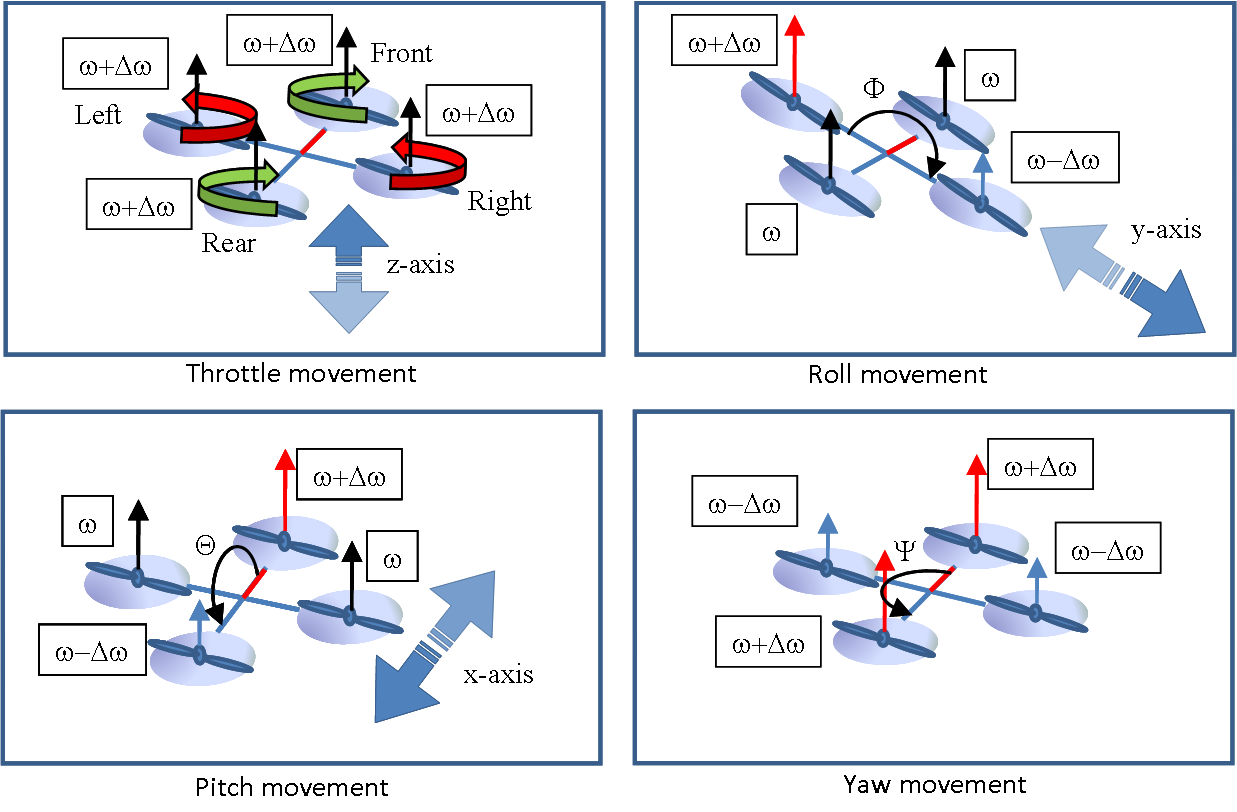
\includegraphics[width=0.75\textwidth]{graphic/QuadrotoDOF.png}
	\caption{Degrees of Freedom of a quadrocopter}
	\label{fig:quadrotoDOF}
\end{figure}

\newpage
To keep the equilibrium of rotational kinematics and to prevent self-rotation,
the motor direction of rotation equals crosswise. The quadrocopter has six \DOF
which can be distinguished as angular and translational movements.
Translational movements can be executed in x-, y- and z- axis. Accelerating all rotors with
the same thrust \ensuremath{\omega} to the value of
\ensuremath{\Delta}\ensuremath{\omega}  will affect a movement in z-direction.
Movements to the negative direction of the z-axis are possible, if the thrust of
the four rotors is smaller as the gravitational force of the aerial vehicle.

 The roll movements can be described as a change of the angle around the x-axis.
Thereby the left and right rotors execute a force difference by slowing down
the one and simultaneous increasing the other thrust with
\ensuremath{\Delta}\ensuremath{\omega}. Related to the thrust difference and angular
 movement, the aerial vehicle creates a force to the y-axis. Equivalent to roll,
 the pitch movement is executed with a change of the angle around the y-axis.
 Also the pitch movement creates a translational
movement across the x-axis. Pitch and roll can only reach a stable angular state
and accelerate to the x- or y-axis, if the value of
\ensuremath{\Delta}\ensuremath{\omega} 
is the same at the diagonal rotors. Otherwise, the quadrocopter would pure rotate
across the corresponding axis.

 The yaw movement is a rotation around the z-axis.
This angular movement results in combination of pairwise different thrusts and
takes as long as the thrusts are different
 \citebib[p.p.8-11 Quadrotor model and system]{CasLozAle05}.
\newline
Synthesizing the weaknesses of \MEMS like noise or the limited resolution,
together with the characteristics of the kinematics of the quadrocopter shows
the problems which come up in case of \MAV control with a \IMU with \MEMS. As
mentioned smoothly accelerations could be a drawback for the control system,
because this kind of accelerations gets lost in the sensor noise.
\newpage
 Regarding the kinematics of the quadrocopter, we have seen that translational
 movements can only be reached with angular movements across the x- and y-axis of with
increasing or decreasing the thrust on every rotor in the z-axis. Imprecise
noisy sensors would affect a wrong thrust regulation at the actuators. Thereby
it is highly improbable, that all four rotors affected by the noise equal and
accelerate in the z-axis. More probable as a uncontrollable acceleration in the
direction of the z-axis, is that pairwise two rotors have the some drift and
create so an unexpected yaw rotation. Finally the most probable will be a
wrong thrust regulation at one rotor, but for a short time interval. So the most
likely error drifts will exist at the x- and y-axis. So the hovering state will
be nearly impossible to reach just with \MEMS acceleration sensors, because the
x- and y- movements have to be zero. 

The following figure \ref{fig:ImpactOfNoise} shows the described problem area
 of \MEMS sensors in the concrete case of the sensors which are mounted at the
quadrocopter \CCU of the \HSE. The mechanical characteristics of the translational acceleration sensor
\citebib [pp.37-39 Typical performance characteristics]{ST05_1}
were simulated under consideration of the change of the position of the
quadrocopter and the applied acceleration.\newpage We can see, that
accelerations which are small enough, get lost in the sensor noise and are invisible for the
quadrocopter. Furthermore the quadrocopter reacts in t=12 if the
acceleration transcends the threshold value of the sensor noise.


\begin{figure}[!htbp]
	\centering
		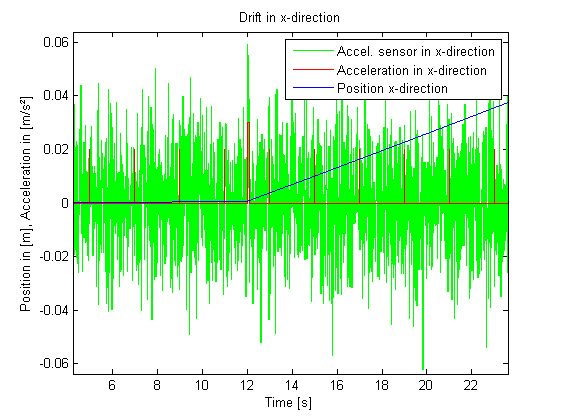
\includegraphics[width=0.75\textwidth]{graphic/ImpactOfNoise.png}
	\caption{The impact of sensor noise}
	\label{fig:ImpactOfNoise}
\end{figure}

% -----------------------------------------------------------------------------------------
\chapter{Initial Survey}

An enormous quantity of researches, which is sponsored by industry companies or
universities, was executed to find a better approach to stabilize \UAV by
using different sensors. Movement detection approaches, which are ultrasonic, sonar or
\RF based, show that it is necessary to have known reference points to get a
reliable result 
\citebib[p.2 Ultrasound indoor localization with reference points]
{EckDreGer09}\citebib[pp.4-5 Radio Model Localization]{BulHeiEst02}.
 The problem of this approach is that the environment has to be prepared before
 the UAV flight.
 This preparation is a drawback in point of flexibility in different operation
 places. Anyway, approaches with ultrasonic, \RF or sonar sensors show that the
 localization of \UAV needs a kind of global feedback to correct the \UAV 
 absolute position. One of the first motivations for a vision based sensor was
 presented by Ettlinger et al. 
 \citebib[pp.1-2 Visual-Based Localization and Control]{EttNecIfjWas04}.
 In this paper, the authors suggest, that vision is the only practical solution
 for obstacles of flight stability and showed an On-board
approach for a \GUAV by detecting the horizon with a forward looking camera and
estimating and control the flight attitude. Further vision based attitude control
approaches also were used for \HUAV with the difference of a down looking
camera for reference point free movement detection or an Off-Board camera which
tracks the global position of the \UAV.


\section{On- vs. Off-Board Camera and Image Processing}

The Off-Board camera approach was researched by Altug et al.
\citebib[p.76 Localization and Control with an Off-Board camera]{AltOstMah02},
 with the result of a less sensitive feature detection and position localization
 as the On-Board camera approach. Off-Board camera tracking is also shown in the
developments of extremely reliable and precise localization of a \UAV and it is
actually used in the development of aggressive autonomous flights of multiple
\MAV in the experiments of Mellinger et al. 
\citebib[Trajectory Generation and Control with Off-Board cameras]
{MelMicKum10} \citebib[pp.363-364]{GurStuAchDotHirRus07}. The advantage of
the Off-Board camera tracking system is that the image capturing and position
tracking is executed outside the \UAV and prevents complex On-Board calculations
for movement and position estimation. The drawbacks of this Off-Board Tracking
methods are that they need a previous prepared testbed for the flying
environment, which is build up with a motion tracking system 
\citebib[pp.1-2 The GRASP Testbed]{MicMelLinKum10}.

Problems, such as a limited power resource, a poor level of algorithm complexity
for image processing resulting from the limited calculating On-Board performance
and the endeavour to economise weight, lead to outsourcing the image processing
to a remote system which is not concerned to the On-Board problems. Langer et al.
\citebib[pp.5-7 Off-Board Image Processing]{LanSuePro08} uses an Off-Board image
processing to track a landing pad for autonomous landing. Thereby the images are
transmitted in this approach over Wifi communication to a base station, which
tracks the landing pad and sends back information of position control. Thereby it was
shown that the landing algorithm has to run at maximal 100Hz to work with
the transmitting delays of the images.\newpage
 This landing algorithm shows that it is possible to outsource successfully the
 image processing in consideration of the sample rate which the algorithm needs.
By regarding the drawback of the image transmission delay of the Off-Board image
processing, On-Board approaches were developed with the focus to the Real-Time
behaviour. Tippetts \citebib[pp.21-22 On-Board image processing with an FPGA]
{Tip08} realized an On-Board approach with a \FPGA which uses a complex feature
tracking algorithm but runs with 100MHz sampling rate. The characteristics
of the feature tracking with a \FPGA can result a fast movement tracking method,
but it is not an efficient method in the behaviour of power consumption because
the hardware is not optimized for the image processing tasks.

%01.11.2010 Stoped here
\begin{figure}[!htbp]
	\centering
		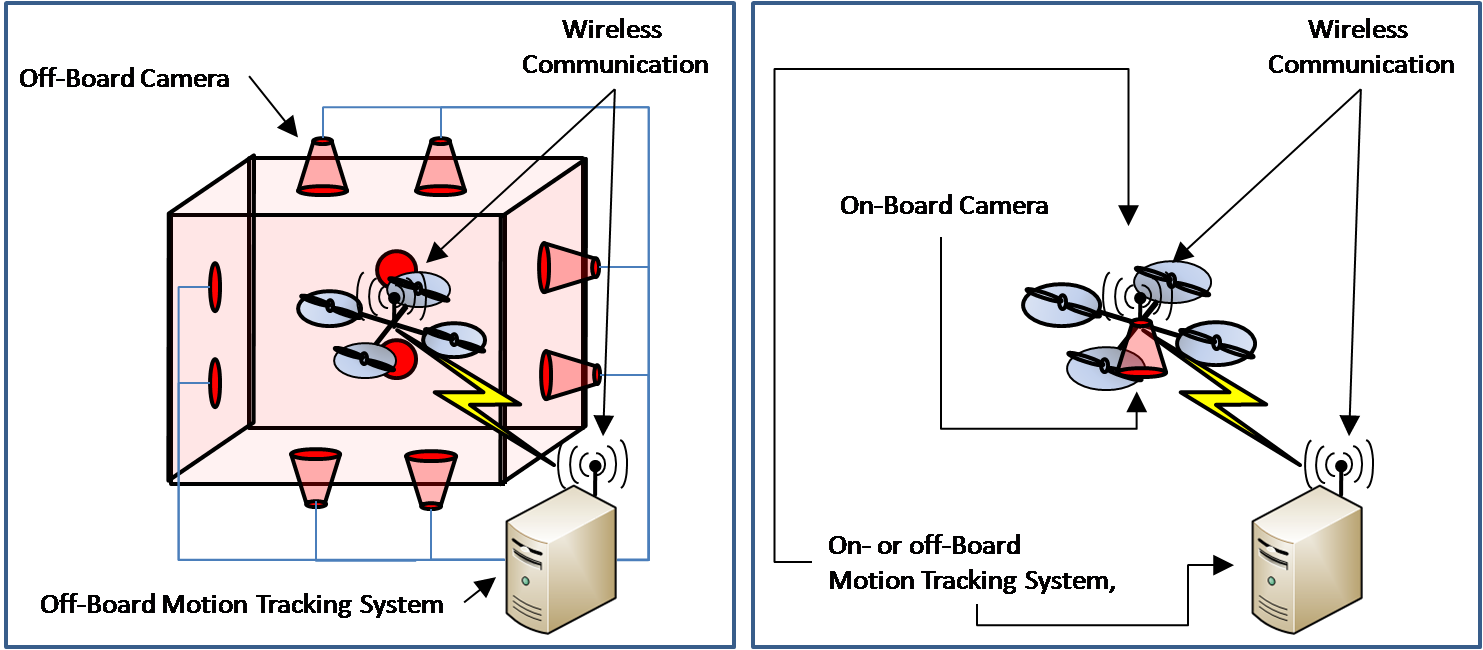
\includegraphics[width=0.85\textwidth]{graphic/Off-BoardvsOn-BoardCameras.png}
	\caption{On- and Off-Board camera and motion tracking system approach}
	\label{fig:Off-BoardvsOn-BoardCameras.png}
\end{figure}

\section{Hardware vs. Software-based image processing}

 In contrast to the drawbacks of \FPGA s, Langer et al.
\citebib[On-Board image processing with mice sensors]{LanSuePro09} and
 Beyeler et al. \citebib[pp.4-5]{BeyChrFlo09} showed an approach for detecting
 the spatial movement of a \UAV with optical mice sensors which have an optimized
 hardware for image processing and are lightweight.
 \newpage
 These sensors calculate the optical flow of the captured images and estimates
 the movement direction of the \UAV in hardware and
can provide a high sample rate. In contrast to the fast movement detection,
a disadvantage, is that these sensors have limitations related to the operating
environments. These limitations are the concrete light and distance range which
is required from the manufacturer 
\citebib[pp.7-15 Limitations of the operating environment] 
{ST05_1}. The most of the experiments with a stabilisation approach with mice
sensors uses optical lens to reach a higher degree of operating distance, but the
effort in most of the cases is not satisfactorily to the results as Langer et.
al have shown
 \citebib [p.6 Performance of the optical flow based position controller] 
 {LanSuePro09}. Software based image processing approaches have a more flexible
 extension and change behaviour, but they work not as fast as hardware based
 approaches. Further advantages of software based image processing are, that the
most of the commercial and open source computer vision \API also provide
implemented estimators and filters to correct the captured input and to decrease
noise of the images. Stowers et al. realized a heading estimation for a
quadrocopter with an onboard \SBC which runs the open source computer vision
toolkit OpenCV\citebib[The OpenCV Reference]{OpenCV2_0}. This software based
image processing approach shows strengths in the modularity of the image processing architecture and in the interchangeability
of the vision system \citebib [pp.1-6 Software Based Vision Processing]
{StoBaiHayMil09}\citebib[Software Structure and Porability]{GarKae08}.

\newpage
\section{Vision based movement detection approaches}

Sequential captured images contain a huge amount of information about the
absolute and relative movement of objects in every direction. So several vision
based movement detection approaches were researched in the topic of \UAV
stabili- sation with different requirements to the information which extracted
from the vision process. A simple approach for a relative vision based control of
a \UAV was implemented by Boabdallah \citebib[pp.110-114 Position Sensor]{Bou07}
by using a down looking camera and the Canny edge detector \citebib{Can86} and
the Douglas Peuker Algorithm for curve equalisation \citebib{DouPeu73}. The drawback of this approach is that the field of vision must contain forms with edges which mean that the approach cannot result a satisfactory result if no
edges are detected. A further approach for detecting relative movements and to
build up a map for autonomous navigation, is visual \SLAM. This approach tracks
features in the field of vision and reconstructs a relation to tracked features
of previous images. The realization of \SLAM \citebib{WilKleRei07} in a \UAV
was executed in the work of Bloesch et al. \citebib{BloWeiScaSie10} under
consideration of real-time characteristics. The behaviour of the algorithm shows
that the localization of the tracked features and the simultaneous mapping has a
big impact at the time delay of the calculation. So the experiments and the
control algorithms were researched and designed for 7.5Hz sample rate. Another
popular tracking method for movement detection is given with the Optical Flow,
which can be described as movement observation of tracked objects or pixels in a
sequence of images. Algorithms to calculate the Optical Flow were introduced by
Horn and Schunk \citebib{HorSch80}, Lukas and Kanade \citebib{LucKan81}.
\newpage A few years after introducing the Lucas-Kanade-Algorithm, Lucas
described the theoretical approach of visual navigation by using the Optical Flow. Thereby he
described the possibility to detect movements and to calculate correspondence
velocities. These velocities can be combined to a vector field which can describe
movements in every direction 
\citebib[pp.40-45 Optical Navigation Theory]{Luc84}.


\begin{figure}[!htbp]
	\centering
		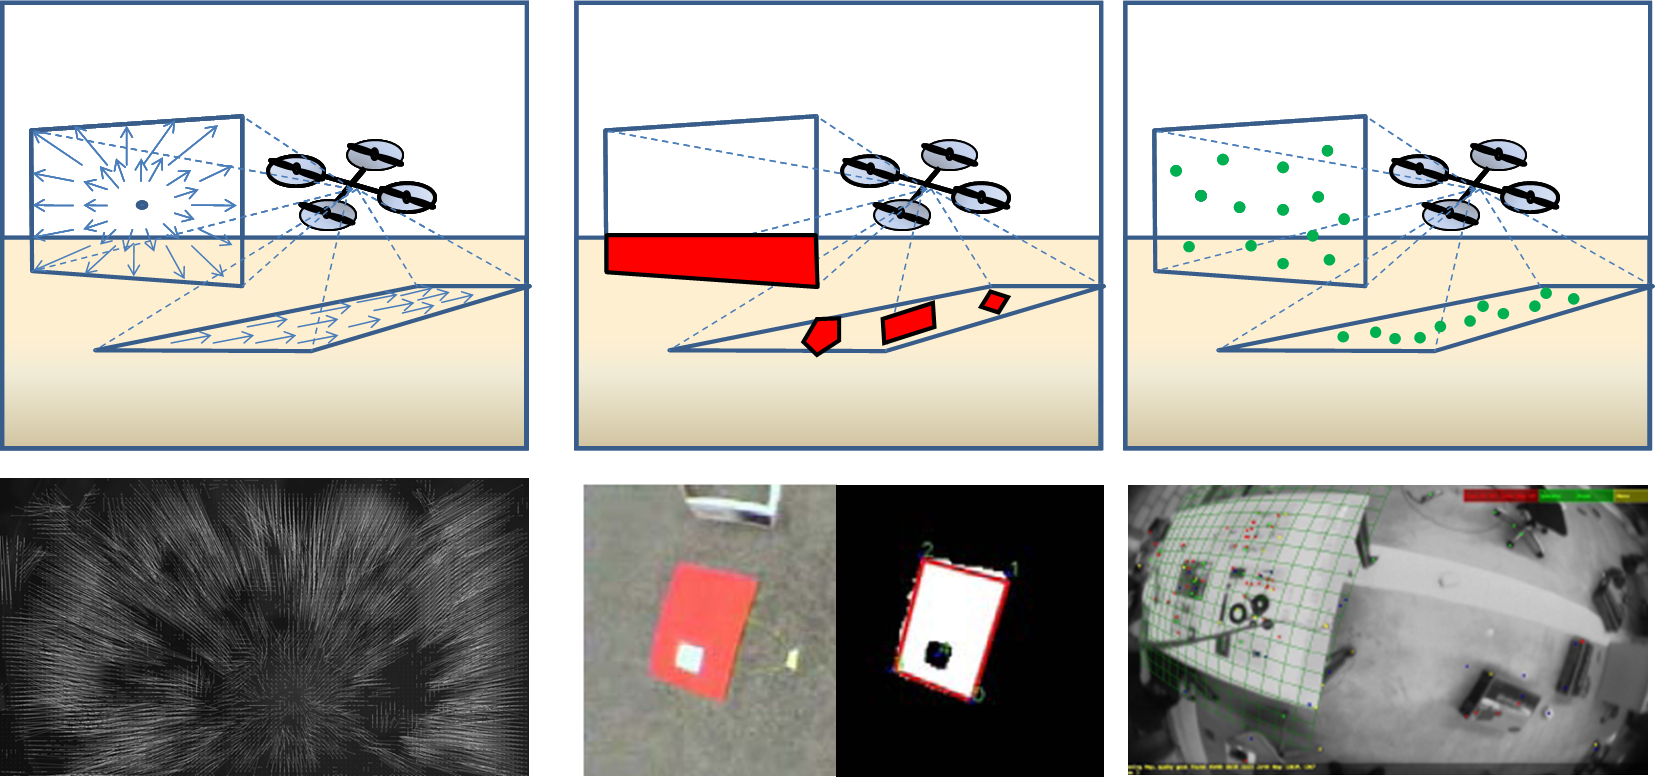
\includegraphics[width=0.75\textwidth]{graphic/VisualApproaches.png}
	\caption{Samples for UAV stabilisation with Optical Flow, Edge detection and SLAM}
	\label{fig:VisualApproaches.png}
\end{figure}

\newpage
\section{Control Approaches}

The closed loop feedback architecture is an approved method for controlling
systems and nearly used in the most of the systems controls in industry and
society. So the most of the researches in the \UAV stabilisation topic were
and still are executed with closed loop control architectures which are built up as
\MIMO systems. The differences between the researched approaches are the
amount of the inputs and outputs of the physical process, the type of controller,
the used measurements and the sampling rate. Thereby the type and behaviour of
the controller is close related to the measurements and the physical process
\citebib[p.3]{DorBis01}.
 The classical control approach using \PID controler was
researched in several \HUAV projects \citebib[pp.24-31]{Sik08}
\citebib[pp.43-68] {Bou07}. These researches show that the \PID control is not
robust enough to handle with measurement errors and to control multiple \DOF s. So the most of
the released control approaches with \PID technique extends the control architecture
with estimators and filters to get more precise measurements. Another
approach for control improvement was introduced by Luenberger \citebib{Lue71} and
describes a closed loop control approach, called state-observer, which simulates
the process in real time parallel to the true process by using the input and
output vector of the closed loop system and corrects the control strategy.
Bloesch et al. \citebib[p.5] {BloWeiScaSie10} have shown in their research,
that the problematic of sensors with non-negligible time delay can be solved to an
adequate result by using a state-observer.\newpage The reason for that is that
the state-observer allows configurate and to control the stability behaviour of the
closed loop feedback architecture. If a process can be observed or furthermore
controlled, is related to the states in which it can be and furthermore to
 the measurements of the \DOF 
 \citebib [pp.632-636 Controllability and Observability]{DorBis01}. In this
 project it has to be determined how correction values which are provided
 from the optical sensor with a slower sampling rate, can include into the
 control algorithm of the aircraft.


\begin{figure}[!htbp]
	\centering
		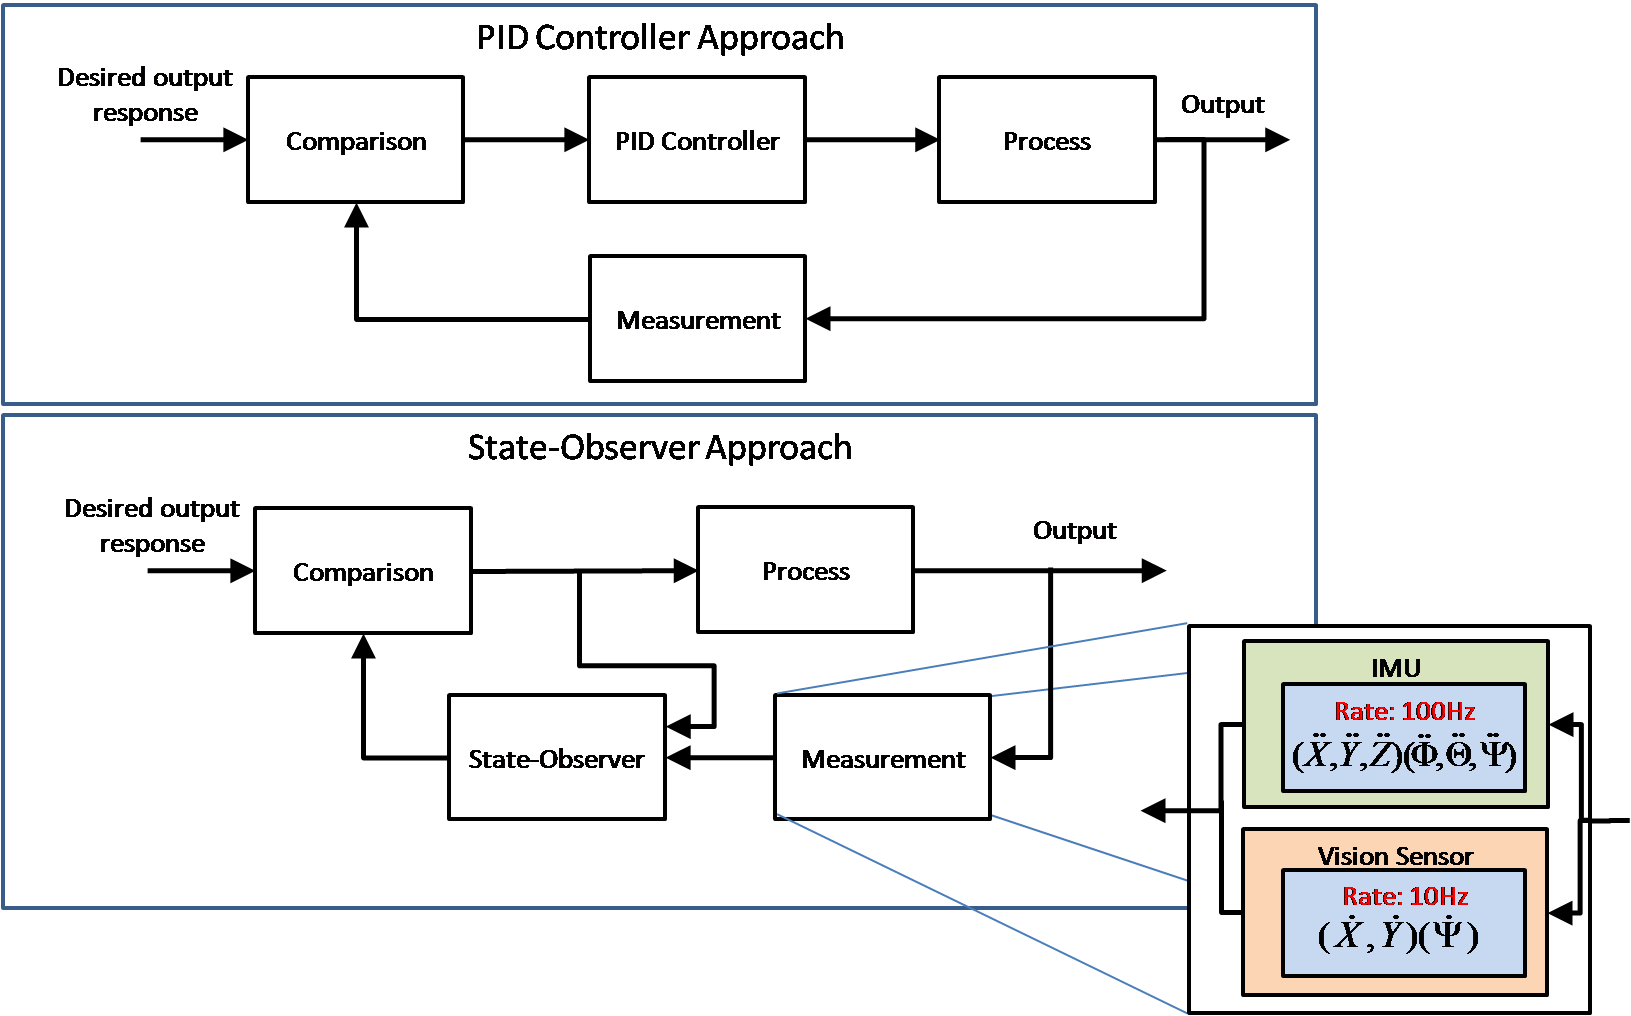
\includegraphics[width=0.75\textwidth]{graphic/ClosedLoopControlSyst.png}
\caption
{PID-Controler and State-Observer in closed loop System with variable sample sensor rates}
	\label{fig:ClosedLoopControlSyst.png}
\end{figure}

\newpage
\section{Proposed Approach}

This chapter shows several approaches for movement detection and stabilisation of
\UAV. The found methods were critically analyzed and assessed with the result
to investigate the following techniques which are shown in figure \ref{fig:ProposedApproach.png}.
 The proposed solution to eliminate the stabilisation problems of the
 quarocopter has to be vision-based for achieving the goal of flexibility and independence of
operational environment. Related to the off-board image processing, the problem
of the processing delay, could be solved with a state-observer. Furthermore the
optical movement detection should work without reference points.
 So the optical flow method has to be researched by using a
software-based detection approach for more flexibility and replaceability.
Because the approach of the flight control is teleoperated and the flight
stabilisation does not have to provide aggressive flight maneuvers, it is simpler
to realize the camera view on-board. This proposed solution has to be simulated
 to check the feasibility and to determine the limitations.


\begin{figure}[!htbp]
	\centering
		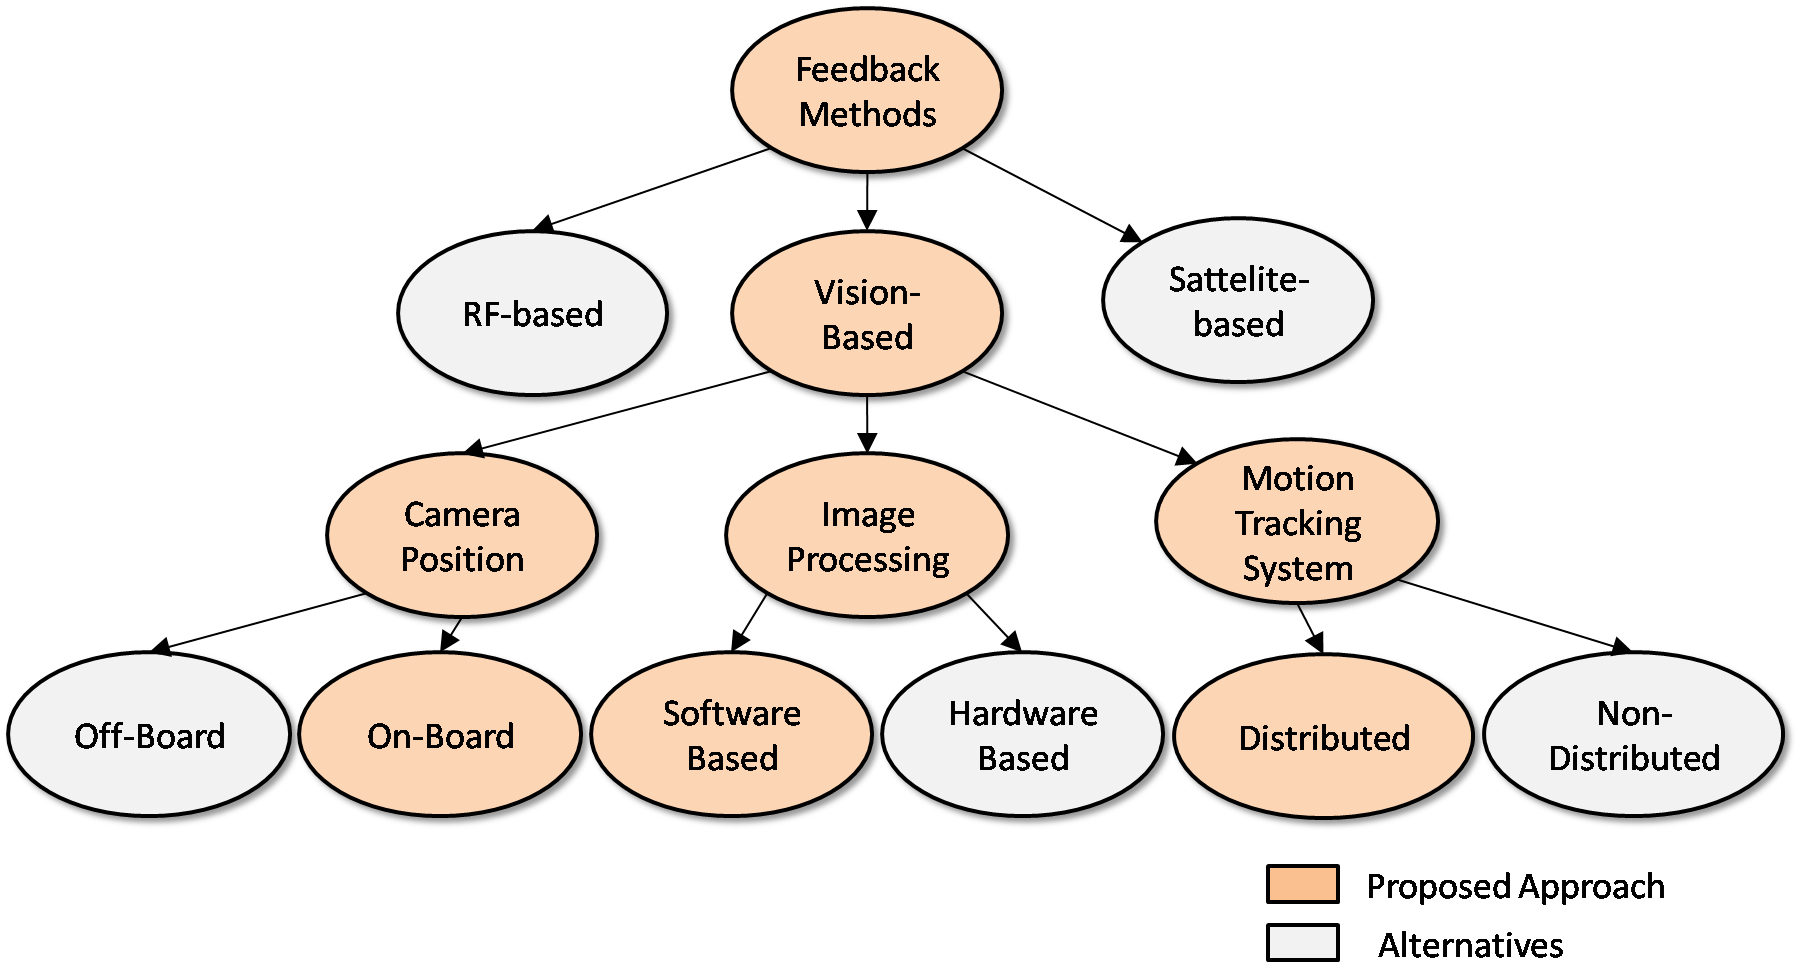
\includegraphics[width=0.75\textwidth]{graphic/ProposedApproach.png}
\caption
{Proposed Approach}
	\label{fig:ProposedApproach.png}
\end{figure}

% -----------------------------------------------------------------------------------------
\chapter{Aims and Objectives}

The aim of this dissertation is to provide a simulation architecture that can be
used as prototype development platform for a distributed visual movement
detection and control of a quadrocopter. Furthermore the characteristics of the
distributed image processing and movement detection have to be analyzed in
relation to the variation of configurations and critically assessed.

One essential objective is that the configuration of the simulating components
provides the option to simulate a range of hardware components which are not
purchased until now. By way of example the simulation of the on-Board camera has
to provide options of configuration for the resolution, color intensity, blur and
so far. The simulation of the communication between \UAV and host also has to
provide a variation of transmission rate and further behaviour which could affect
the visual movement detection at the base station. The efficiency in relation
with the quality of function is an important indicator for the success and acceptance of
the distributed movement detection approach. So it is important to get an insight
to the possible characteristics of the simulated components with the result to
find a way which satisfies the efficiency and quality aspects.

Another important objective is that the interfaces between the simulating
components are clearly specified and allow a way of modular exchangeability of
simulation components with the real objects.\newpage This purpose has to allow a
more precise investigation of the behaviour of the real hardware related components
and the option to test software for the \UAV target, like the On-Board control
algorithm, at the base station.

The realization of the simulation therefore has to provide an encapsulated and
flexible architecture and has to simulate behaviour like delays and jitters for
simulated components. Thereby the simulation has to adjust a real-time-behaviour
in the complete simulated environment and to allow so measurements and prediction
of feasibilities with the simulated configuration.

% -----------------------------------------------------------------------------------------
\chapter{Experimental and Investigative Methods}

\section{Development Process}

During the initial survey we have seen many approaches for aircraft stability and
movement detection of \UAV. The most of these approaches were developed
iterative under consideration of the upcoming problems and obstacles 
\citebib[Iterative Development, Single and Dual Camera Feedback]
{AltOstMah02, AltOstTay03}
\citebib[Iterative Development, Landing and Position Control Development]
{LanSuePro08, LanSuePro09}. This procedure model also will be appropriate to this project, because the potential risks are difficult to identify. So the outcome of the development process have to be a
prototype which can be evaluated, tested and extended. A process model, which
provides an appropriate structure to face the iterative prototyping strategy
under the consideration of the risk aspects, is given with the spiral model. The
classical spiral model has typically four phases in which the product is
developed in an incremental evolutionary process. Derivates of this classical
model which focus the customer evaluation for quality improvements may three,
five or six phases. In the context of this project, the classical four phases
spiral model is used for scientific and feasibility study and does not have to
provide further customer communication phases
\citebib[pp.36-38 The Spiral Model]{Pre01}.

\newpage
A typical cycle of the four phases spiral model (\ref{fig:SpiralModelAndMBD})
 begins with the identification of
the objectives which have to be elaborated like performance,
functionality, flexibility and so far. The next step is to evaluate the
alternatives relative to the objectives and constraints and to determine
significant sources of risks. After that, the next level
iteration of the product is planned. In the special case of this project it is
comfortable to use \MBD in this phase by using the results of the previous phase as input.
This input can be a planed prototype or requirements which describe the changes
to execute. The output of the \MBD phase can be used again in the planning phase
for the next iteration \citebib
[pp.64-69 Spiral Model of the Software Process]{Boe88}.


\begin{figure}[!htbp]
	\centering
		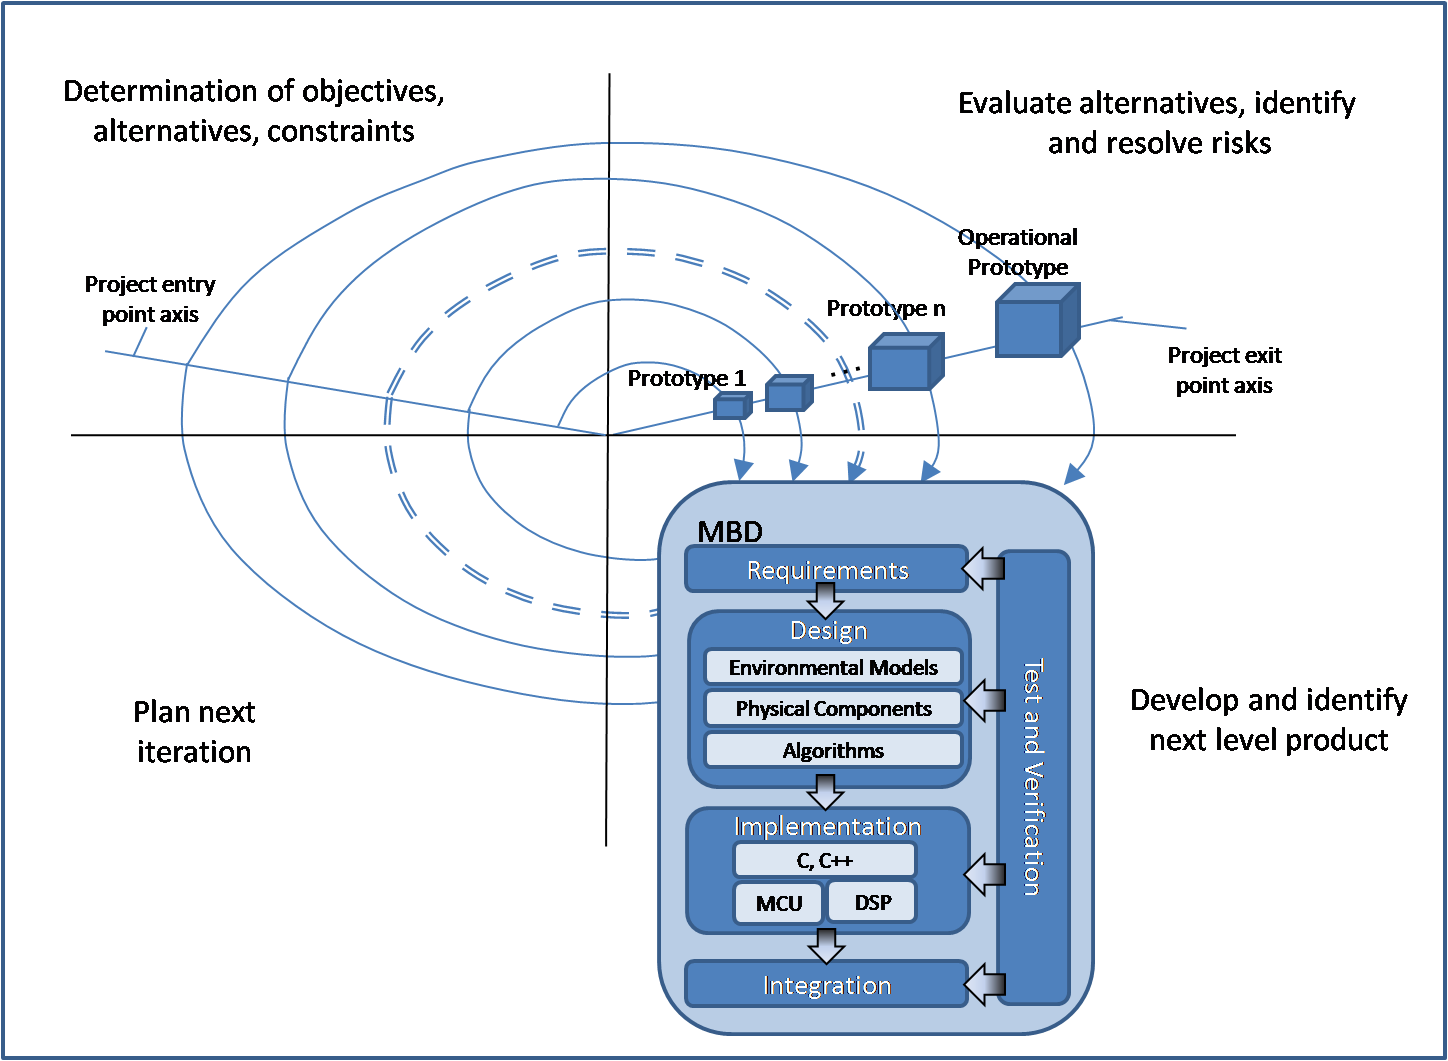
\includegraphics[width=0.75\textwidth]{graphic/SpiralModelAndMBD.png}
\caption
{The Spiral Model in combination with Model Based Design}
	\label{fig:SpiralModelAndMBD}
\end{figure}

\newpage
\section{Model Based Design}

\MBD is a popular method to encounter problems which come up in the development
of mechatronic products. These systems almost involve mechanical, electrical, control
 and embedded components which are developed in different teams of
engineers with a specialized focus on the part of the complete project. Some of
these components are related on the results of other components before they can
be developed. This problem can be solved with Model Based Design and the
advantage to develop modules of the complete project by simulating their
environment. So the development can run highly parallel with the benefit that the
modules can be continuous tested in each phase of the project
\citebib[pp.1-2 Challenges of mechatronic product development]{EasLamTur09}.

The development section in figure \ref{fig:SpiralModelAndMBD} includes the phases
and the corresponding key capabilities of \MBD. The first phase of \MBD is the
realization of the researched and required components into a simulation
environment. Thereby physical components, environmental model and algorithms are
abstracted to systems by using domain-specific modeling tools with a well
defined edges and intercommunication. The developed systems in the design phase
can be tested simultaneously to analyze the system performance and correctness.
Other key capabilities of \MBD are given in the implementation phase. The \MBD
tool Matlab allows to generate embedded code from the designed systems or to
combine handwritten code with the build simulation of the design phase. So the
implemented modules can be similarly tested in the adopted simulation
environment. Finally components which have passed the tests at the implementation
phase can be integrated together.\newpage Ultimately the final product can also be tested
with the \MBD tool by simulating the environment of the product e.g. in a \HIL
test bench. \citebib[Model Based Design, MathWorks]{Mat10}

\section{Overall Design Model}
The overall design model gives an overview of the components of the simulation
which has to be realized in the context of this project and the corresponding
applied techniques. As visualised in figure \ref{fig:InitialDesign}, the left
side of the simulation abstracts the embedded system of the quadrocopter. Inside
these components the plant or physical model has to simulate the movement
behaviour in the \DOF of the quadrocopter. Furthermore the controller has to
correct the position of the \UAV and to compensate outside disturbances with
information of the \IMU and the distributed correction value of the base station.
The environment simulation which has to include the underground and disturbances
simulation will be triggered to start just as the rest of the simulation with a
task which describes the ideal flight manoeuvre. The transmissions of the camera
\IMU and correction data have to be delayed in relation to a configurable
transmission rate. The image processing has to be executed with an application,
realized in OpenCV \citebib[OpenCV Project]{OpenCV2_0} and invoked by Matlab
\citebib[OpenCV and MEX-Functions in Matlab]{EsmSna08}. The calculated drift from
image processing finally has to be compared with the received values of the \IMU
to determine the position correction value. This correction has to be
transmitted to the embedded system and included in the correction of the controller.
\newpage
 The novel aspect of the project here is reflected in the approach to simulate
 the complete embedded system, the transmission process, the base station and to realize the
image processing in an application. The strength of this approach is that the
simulation gives better results and a deep insight to the concurrent processes
and helps to understand the challenges and limitations of the investigated
scheme.


\begin{figure}[!htbp]
	\centering
		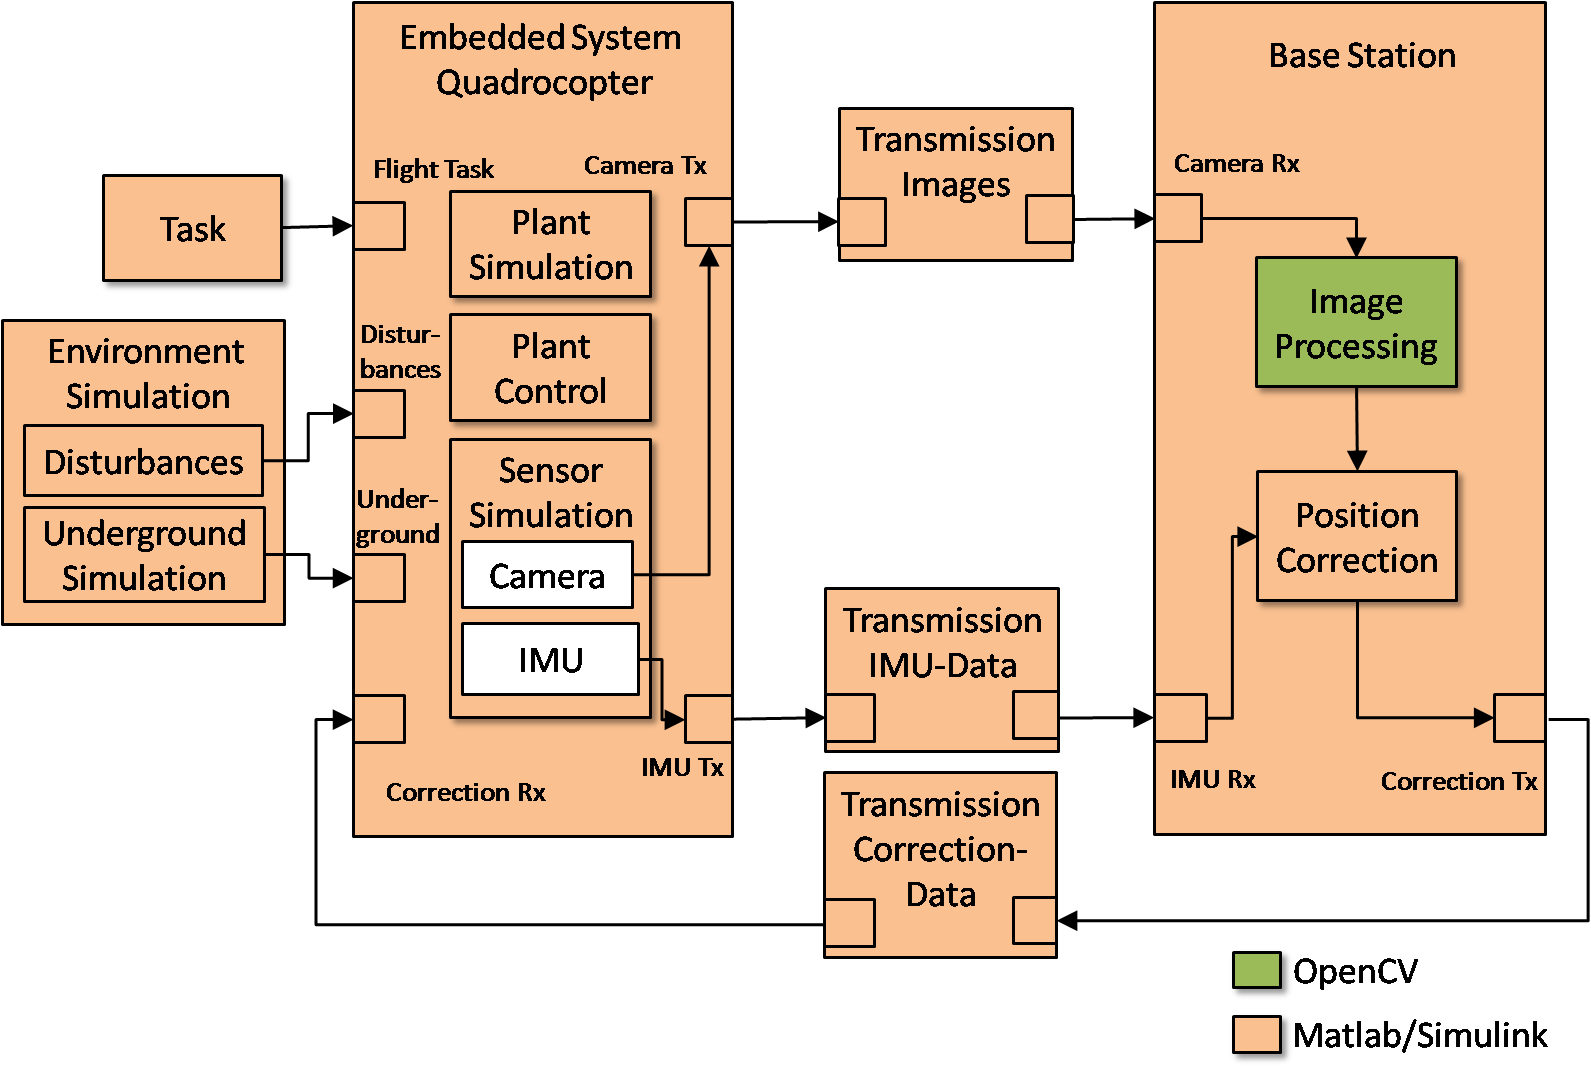
\includegraphics[width=0.75\textwidth]{graphic/InitialDesign.png}
\caption
{The Overall Design Model of the Simulation}
	\label{fig:InitialDesign}
\end{figure}


% -----------------------------------------------------------------------------------------
\chapter{Project Plan}

The Project Plan of this Master's Dissertation is visualized in figure
\ref{fig:ProjectPlan}. The critical, red path is the result of the
parallelization of some work packages. These packages mostly are independent and
include idle time delays, so that it is more efficient to parallelise them. For 
example we can regard the simulation and research together with the Master's Thesis documentation. These work packages can be parallelized, because the
simulations which have to be executed are time intensive and not a basic part of
the complete documentation. Furthermore we can see that one cycle of the spiral
model will be executed in the context of this Master's Thesis including an
iteration of the \MBD process.

\begin{figure}[!htbp]
	\centering
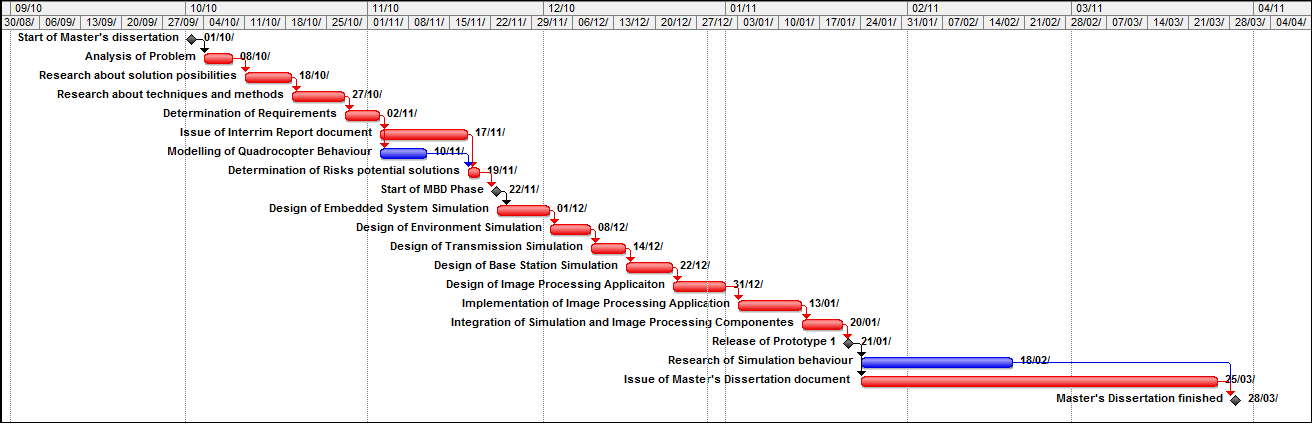
\includegraphics[width=1.1\textwidth, height=180px]{graphic/ProjectPlan.png}
\caption
{The Project Plan}
	\label{fig:ProjectPlan}
\end{figure}

% -----------------------------------------------------------------------------------------
\chapter{Deliverables and Outcomes}

The expected outcome of the Master's Thesis is the research and feasibility study
of the distributed position correction scheme which has to reflect the
improvements of drift eliminations. This has to be realized with a simulation
prototype which reflects behaviour of the real components and allows a look
insight the complete system. Another outcome has to be the image processing
application at the base station which has to collaborate with the simulation.


% -----------------------------------------------------------------------------------------
% ############################################################################################


% Alle Eintr�ge der BibTeX Datenbank "zitieren"
%\nocitebib*
%\nociteref*

% Auswahl der BibTeX Datenbank f�r das Literaturverzeichnis
%Dio: habe die References entfernt
%\bibliographyref{literature/literatur}
%\bibliographystyleref{plain}

\bibliographybib{literature/literatur}
\bibliographystylebib{alpha}

%\bibliography{literature/references}
%\bibliography{literature/literatur}

% Einstellen des Bibliography-Stils f�r das Literaturverzeichnis
%\bibliographystyle{plain}

% ------------------------------------------------------------------
% Ausgabe des Wortindex
% idxtotoc Option scheint nicht zu funktionieren
%\clearpage
%\addcontentsline{toc}{chapter}{Index}
%\printindex

% Laut Markus Kohm wird \backmatter normal nicht ben�tigt
%\backmatter
\end{document}

